% Oficina de LaTeX (19.05.2008)
% Autor: Leandro Gutierrez Rizzi
% Exemplo 11

\documentclass[twocolumn,a4,11pt]{article}
\usepackage[T1]{fontenc}
\usepackage[utf8]{inputenc}
\usepackage[brazil]{babel}
\usepackage{epsfig}
\usepackage{amsmath}

\headheight 20mm      %
\oddsidemargin 2.0mm  %
\evensidemargin 2.0mm %
\topmargin -40mm      %
\textheight 250mm     %
\textwidth 160mm      %

\begin{document}

\title{\Large{\bf Estudo numérico da convergência do somatório de Ewald em redes bidimensionais}}

\author{{\bf {\large \underline{Leandro G. Rizzi}}}, {\bf {\large Nelson A. Alves}} \\
 {\small Depto de Física e Matemática, FFCLRP, USP,} \\
 {\small 14040-901, Ribeirão Preto, SP} \\
 {\small E-mail: lerizzi@pg.ffclrp.usp.br, alves@ffclrp.usp.br}}

\date{}

\maketitle

\thispagestyle{empty}

\section{Introdução}

Indentificamos em inúmeras situações a necessidade de efetuarmos somas sobre sítios em redes regulares de tamanho infinito. Dentre as aplicações, citamos os cálculos da energia de interação coulombiana entre cargas em uma rede iônica cristalina e da energia de interação entre dipolos em uma rede de spins. Neste sentido, é conveniente estudar termos de potencial de forma generalizada. Assim, consideremos sistemas cujo potencial de interação entre os seus constituintes seja dado pela expressão
\begin{equation}
U^{(p)}=g \sum_{i=1}^{N} \sum_{j=1}^{N} \sum_{|\vec{n}|=0}^{\infty} {}^{\prime} ~
\frac{q_{i} q_{j}}{ \left| \vec{r}_{ij} + \vec{n} \right|^{p} } ~~~,
\label{utotal_s_s}
\end{equation}
onde $N$ é o número de partículas do sistema, $g$ define a intensidade da interação entre duas partículas $i$ e $j$ que possuem as propriedades físicas intrínsecas $q_{i}$ e $q_{j}$ (e.g. massa, carga elétrica, spin), $r_{ij}=|\vec{r}_{i}-\vec{r}_{j}|$ é a distância entre as duas partículas e $p$ é definido como um número real positivo.

O somatório infinito é inserido no potencial quando consideramos condições de contorno periódicas, onde imagens do sistema são infinitamente replicadas em todas as direções formando uma rede. Efetuamos o somatório sobre as componentes do vetor $\vec{n}$, o qual indica a posição de cada imagem. A notação ${}^{\prime}$ indica que $\vec{n}=0$ é excluído do somatório quando $i=j$, impedindo a auto-interação.

O aparecimento desse somatório nos cálculos da energia nos leva a uma questão prática muito comum em simulações computacionais: a convergência numérica. Séries que possuam convergência lenta aumentam significativamente o custo computacional. Portanto faz-se importante desenvolver métodos que efetivamente aumentem a convergência destas séries.

Interessante observar que este tipo de análise, importante do ponto de vista numérico, teve seu desenvolvimento inicial em 1921 com Paul P. Ewald \cite{EWA}. Neste estudo, Ewald propôs, baseado em argumentos físicos, a transformação do somatório sobre a rede, o qual converge lentamente, em dois outros somatórios. Estes novos somatórios, os quais apresentam uma melhor convergência, são caracterizados por efetuarem somas, quer no espaço real (também chamado de direto), quer no espaço recíproco.

Apresentamos aqui, além de alguns aspectos analíticos do método de Ewald, um estudo numérico sobre a influência do parâmetro de Ewald na convergência das séries.

\section{Aspectos analíticos do método de Ewald}

\noindent
Por uma questão de simplicidade reescrevemos a equação (\ref{utotal_s_s}) da seguinte maneira:
\begin{equation}
U^{(p)}=g \sum_{i=1}^{N} \sum_{j=1}^{N} q_{i} q_{j} S_{ij}^{(p)} ~~~,
\label{utotal_c_s}
\end{equation}
com
\begin{equation}
S_{ij}^{(p)}=\sum_{|\vec{n}|=0}^{\infty} {}^{\prime} ~
\frac{1}{ \left| \vec{r}_{ij} + \vec{n} \right|^{p} } ~~~.
\label{ptotalum}
\end{equation}

Podemos fazer a seguinte decomposição utilizando uma função $f_{p}(\alpha r)$:
\begin{equation}
\frac{1}{r^{p}}=\frac{1-f_{p}(\alpha r)}{r^{p}} + \frac{f_{p}(\alpha r)}{r^{p}} ~~,
\end{equation}
para tanto, devemos impor os seguintes comportamentos para $f_{p}(\alpha r)$:
\begin{eqnarray*}
& \text{i.}  & f_{p}(\alpha r) \rightarrow 1 ~~\text{se}~~ r \rightarrow \infty ~, \\
& \text{ii.} & f_{p}(\alpha r) \rightarrow 0 ~~\text{se}~~ r \rightarrow 0 ~.
\end{eqnarray*}

O parâmetro $\alpha$ no argumento de $f_{p}$ é chamado de parâmetro de convergência de Ewald. Seu valor reflete a rapidez da convergência relativa entre as somas direta e recíproca.

Utilizando a notação $r_{ij,\vec{n}}=\left| \vec{r}_{ij} + \vec{n} \right|$, podemos reescrever a equação (\ref{ptotalum}) como a soma de dois termos,
\begin{equation}
S_{ij}^{(p)}= S_{ij,\text{direta}}^{(p)} + \tilde{S}^{(p)}_{ij} ~~~,
\nonumber
\end{equation}
onde
\begin{equation}
S_{ij,\text{direta}}^{(p)}=\sum_{|\vec{n}|=0}^{\infty} {}^{\prime} ~
\frac{1-f_{p}(\alpha r_{ij,\vec{n}} ) }{
(r_{ij,\vec{n}})^{p} }
\label{gpsomadireta}
\end{equation}
e
\begin{equation}
\tilde{S}^{(p)}_{ij}=\sum_{|\vec{n}|=0}^{\infty} {}^{\prime} ~
 \frac{
f_{p}(\alpha r_{ij,\vec{n}})}{
(r_{ij,\vec{n}})^{p} } ~~ .
\label{gpsomarec}
\end{equation}

A seguir, podemos somar e subtrair o termo quando $\vec{n}=0$ e $i=j$ na equação (\ref{gpsomarec}) de modo a obter
\begin{equation}
\tilde{S}^{(p)}_{ij}=S^{(p)}_{ij,\text{recíproca}}-S_{ij,\text{auto-interação}}^{(p)} ~~ ,
\nonumber
\end{equation}
onde
\begin{equation}
S^{(p)}_{ij,\text{recíproca}} = \sum_{|\vec{n}|=0}^{\infty}
\frac{
f_{p}(\alpha r_{ij,\vec{n}})}{
(r_{ij,\vec{n}})^{p} }
\label{gpsomareciproca}
\end{equation}
e
\begin{equation}
S_{ij,\text{auto-interação}}^{(p)}= \lim_{r_{ij} \rightarrow 0} \frac{
f_{p}(\alpha r_{ij})}
{(r_{ij})^{p} } ~~ .
\label{gpautointeracao}
\end{equation}

\vspace{0.6cm}

A partir do comportamento imposto para $f_{p}(\alpha r)$, podemos defini-la como
\begin{equation}
f_{p}(\alpha r)= \frac{\gamma\left(\frac{p}{2},\alpha^{2} r^{2}\right)}{\Gamma\left(\frac{p}{2}\right)} ~~ ,
\label{gpgammainf}
\end{equation}
onde $\Gamma(\frac{p}{2})$  é a {\it função gama} e $\gamma(\frac{p}{2},\alpha^{2} r^{2} )$ é a {\it função gama incompleta inferior}. 

A Figura \ref{fp} mostra o comportamento de $f_{p}(\alpha r)$ para diferentes valores de $\alpha$ e $p$, com $\alpha=5/L$. Particularizamos nosso estudo para dois casos com importantes aplicações físicas: interações coulombianas ($p=1$) e interações dipolares ($p=3$).

Utilizando as propriedades relacionadas às {\it funções gama} \cite{GRAD}, não é difícil mostrar que
\begin{equation}
1-f_{p}(\alpha r)= \frac{\Gamma\left(\frac{p}{2},\alpha^{2} r^{2}\right)}{\Gamma\left(\frac{p}{2}\right)} ~~ .
\label{gpgammasup}
\end{equation}

\vspace{0.2cm}

\begin{figure}[!ht]
\centering
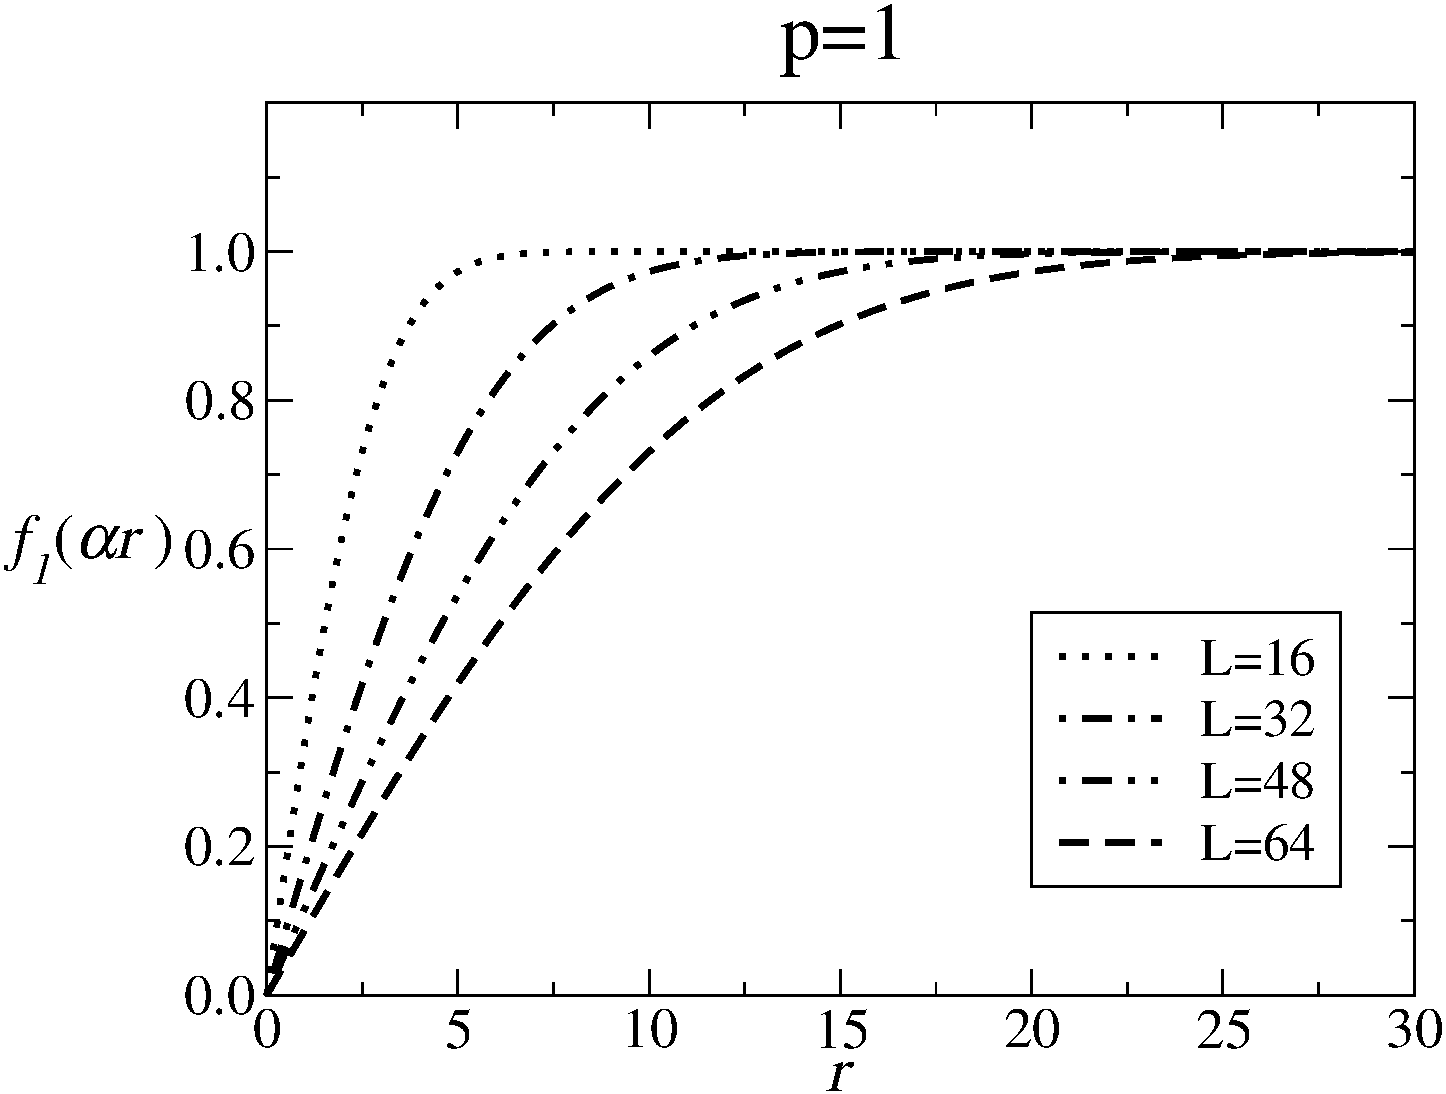
\includegraphics[width=0.5\textwidth]{p1}
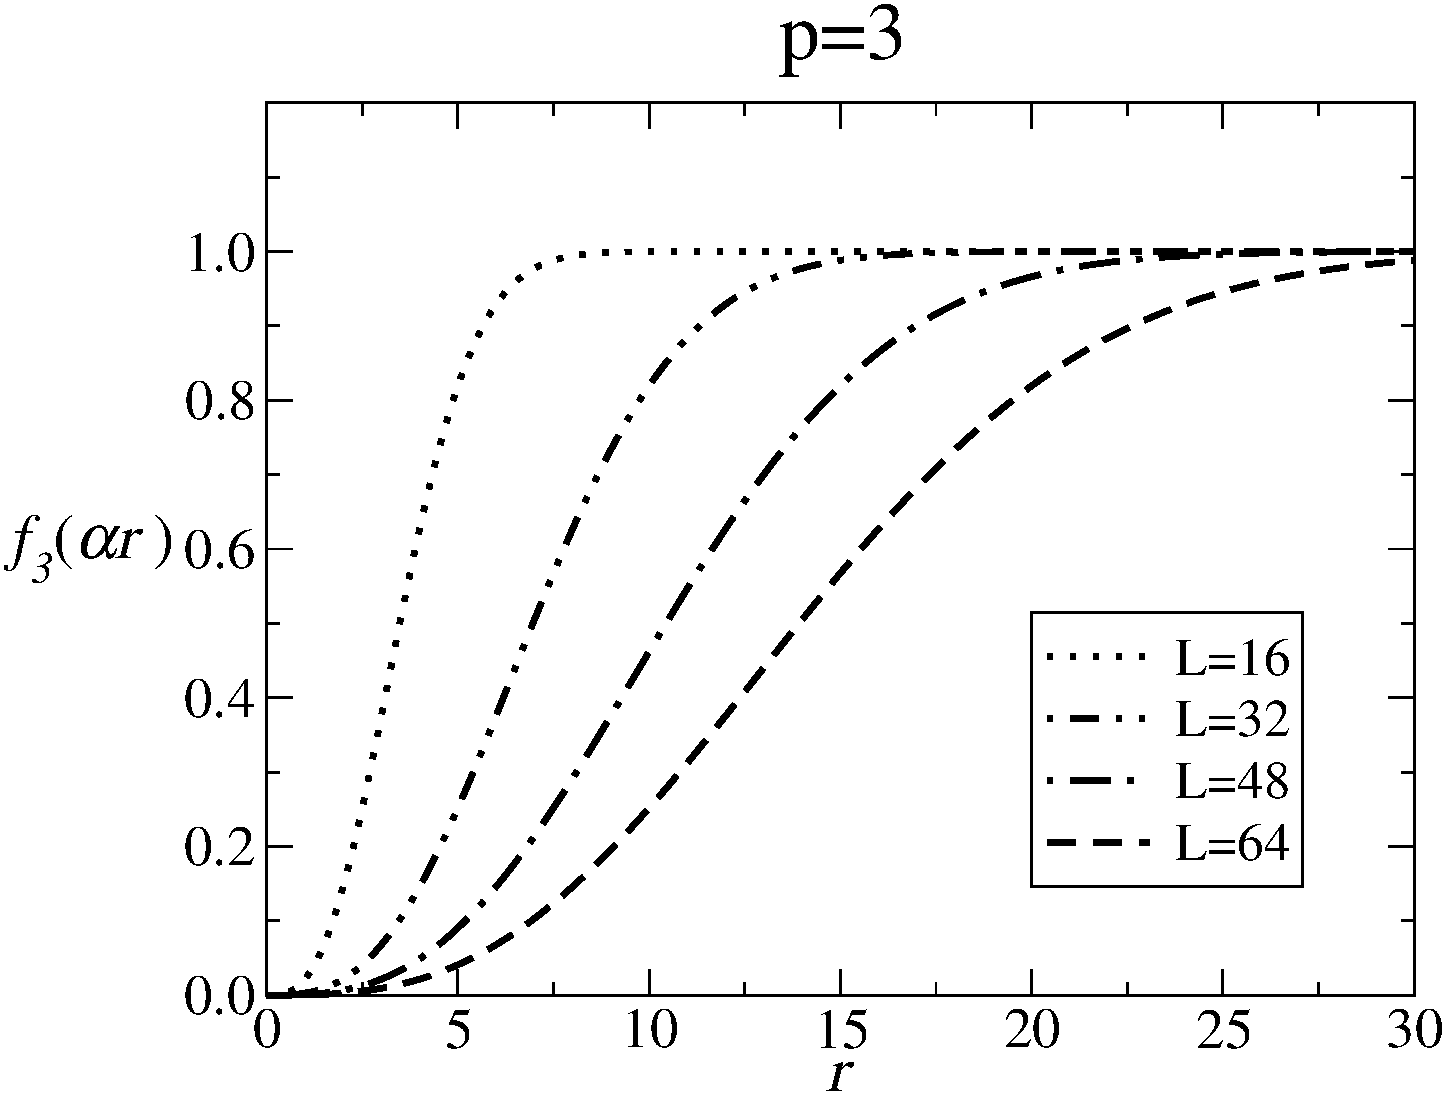
\includegraphics[width=0.5\textwidth]{p3}
\renewcommand{\figurename}{Figura}
\caption{ {\small Gráficos de $f_{p}(\alpha r)$ para diferentes valores de $\alpha=5/L$ e $p$.}}
\label{fp}
\end{figure}

\noindent
{\bf Soma direta}

Substituindo o resultado em (\ref{gpgammasup}) na equação (\ref{gpsomadireta}), obtemos a parte do somatório que consiste numa soma no espaço direto,
\begin{equation}
S_{ij,\text{direta}}^{(p)}=\frac{1}{\Gamma\left(\frac{p}{2}\right) }  \sum_{|\vec{n}|=0}^{\infty} {}^{\prime} ~
\frac{\Gamma\left(\frac{p}{2},\alpha^{2} (r_{ij,\vec{n}})^{2}\right)}
{ (r_{ij,\vec{n}})^{p} }~ .
\label{somadireta}
\end{equation}

\noindent
{\bf Soma recíproca}

De maneira análoga, podemos substituir a definição introduzida em (\ref{gpgammainf}) na equação (\ref{gpsomareciproca}) para obter
\begin{equation}
S^{(p)}_{ij,\text{recíproca}} =\frac{1}{\Gamma\left(\frac{p}{2}\right) }  \sum_{|\vec{n}|=0}^{\infty} \frac{
\gamma\left(\frac{p}{2}, \alpha^{2} (r_{ij,\vec{n}})^{2}\right)}{ 
(r_{ij,\vec{n}})^{p} }~ .
\label{spsomareciproca}
\end{equation}

Fazendo uso da {\it distribuição delta de Dirac} podemos reescrever a equação (\ref{spsomareciproca}) da seguinte forma:
\begin{equation}
S^{(p)}_{ij,\text{recíproca}} =\frac{1}{\Gamma\left(\frac{p}{2}\right) }
\int w(\vec{r})
\frac{\gamma\left(\frac{p}{2}, \alpha^{2} \left| \vec{r} \right|^{2}\right)}{
\left| \vec{r} \right|^{p} } ~ d\vec{r} ~ ,
\label{wsomareciproca}
\end{equation}
onde
\begin{equation}
w(\vec{r})=\sum_{|\vec{n}|=0}^{\infty} \delta(\vec{r}-(\vec{r}_{ij}+\vec{n}))~ .
\nonumber
\end{equation}

Utilizando a relação a seguir (vide referência \cite{NIJ}):
\begin{equation}
\sum_{|\vec{n}|=0}^{\infty} \delta(\vec{r}-(\vec{r}_{ij}+\vec{n}))=
\frac{1}{V} \sum_{|\vec{G}|=0}^{\infty} e^{i \vec{G}.(\vec{r}-\vec{r}_{ij})} ~ ,
\nonumber
\end{equation}
podemos reescrever a equação (\ref{wsomareciproca}) como segue,
\begin{equation}
S^{(p)}_{ij,\text{recíproca}} =
~~~~~~~~~~~~~~~~~~~~~~~~~~~~~~~~~~~~~~~~~~~~
\nonumber \\
\end{equation}
\begin{equation}
\frac{1}{V \Gamma\left(\frac{p}{2}\right) }
\sum_{|\vec{G}|=0}^{\infty}
\left[
\int
\frac{\gamma\left(\frac{p}{2}, \alpha^{2} \left| \vec{r} \right|^{2}\right)}{
\left| \vec{r} \right|^{p} }  e^{i \vec{G}.\vec{r}} d\vec{r} 
\right]
e^{-i \vec{G}.\vec{r}_{ij}} ,
\label{intsomareciproca}
\end{equation}
onde $V=L^{d}$, $L$ é o comprimento do sistema e $d$ é a dimensão espacial. O vetor $\vec{G}=\frac{2 \pi}{L} \vec{k}$ é um vetor no espaço recíproco.

Empregando a relação abaixo (vide referência \cite{GAO}), para $d=2$, na expressão (\ref{intsomareciproca}),
\begin{eqnarray}
\int \frac{\gamma\left(\frac{p}{2},\alpha^{2} \left| \vec{r} \right|^{2}\right)}{r^{p}} ~ e^{i\vec{G}.\vec{r}} d^{2} \vec{r} = ~~~~~~~~~~~~~~~~
\nonumber \\
\pi \left(\frac{G}{2}\right)^{p-2} ~ \Gamma\left(-\frac{p}{2}+1,\frac{G^{2}}{4 \alpha^{2}}\right) ~,
\label{relacaoum}
\end{eqnarray}
chegamos finalmente à expressão para a soma no espaço recíproco:
\begin{equation}
S^{(p)}_{ij,\text{recíproca}} =
~~~~~~~~~~~~~~~~~~~~~~~~~~~~~~~~~~~~~~~~~~~~
\nonumber
\end{equation}
\begin{equation}
\frac{ \pi}{L^{2} \Gamma\left(\frac{p}{2}\right) }
\sum_{|\vec{G}|=0}^{\infty}
\frac{G^{p-2}}{2^{p-2}} ~
\Gamma\left(-\frac{p}{2}+1,\frac{G^{2}}{4 \alpha^{2}}\right)
e^{-i \vec{G}.\vec{r}_{ij}} ~ .
\label{somarecipexp}
\end{equation}

É conveniente eliminar a dependência complexa nesta expressão. Para tal utilizamos a identidade a seguir,
\begin{equation}
\sum_{|\vec{G}|=0}^{\infty} F(G)e^{-i \vec{G}.\vec{r}_{ij}} =
\sum_{|\vec{G}|=0}^{\infty} F(G)\cos(\vec{G}.\vec{r}_{ij}) ~ .
\nonumber
\end{equation}

Assim, podemos reescrever a equação (\ref{somarecipexp}) como:
\begin{equation}
S^{(p)}_{ij,\text{recíproca}} = \frac{ \pi}{L^{2} \Gamma\left(\frac{p}{2}\right) }
~~~~~~~~~~~~~~~~~~~~~~~~~~~~~
\nonumber
\end{equation}
\begin{equation}
\sum_{|\vec{G}|=0}^{\infty}
\frac{G^{p-2}}{2^{p-2}} ~
\Gamma\left(-\frac{p}{2}+1,\frac{G^{2}}{4 \alpha^{2}}\right)
\cos(\vec{G}.\vec{r}_{ij}) .
\label{somareciproca}
\end{equation}

Enfatizamos que esta última expressão, bem como a relação (\ref{relacaoum}) e a expressão (\ref{somarecipexp}), são exclusivas para redes bidimensionais, sendo as demais gerais para qualquer dimensão espacial.\\


\noindent
{\bf Auto-interação}

Por último, substituindo a definição (\ref{gpgammainf}) na expressão (\ref{gpautointeracao}) obtemos
\begin{equation}
\label{autolimiter}
S_{ij,\text{auto-interação}}^{(p)}=\frac{1}{\Gamma\left(\frac{p}{2}\right) }  \lim_{r_{ij} \rightarrow 0} \frac{
 \gamma\left(\frac{p}{2},\alpha^{2} r_{ij}^{2}\right)}{
r_{ij}^{p} } ~ .
\end{equation}

Fazendo a mudança de variável $x=\alpha^{2} r_{ij}^{2}$ e observando que:
\begin{eqnarray*}
& \text{i.} &
\lim_{r_{ij} \rightarrow 0}  \gamma\left(\frac{p}{2},\alpha^{2} r_{ij}^{2}\right)=\lim_{x \rightarrow 0}  \gamma\left(\frac{p}{2},x\right) = 0 ~,
\\
& \text{ii.} &
\lim_{r_{ij} \rightarrow 0} r_{ij}^{p}=\lim_{x \rightarrow 0} \frac {x^{\frac{p}{2}}}{\alpha^{p}} = 0 ~,
\end{eqnarray*}
podemos calcular o limite na equação (\ref{autolimiter}) através da regra de L'Hopital. Assim,
\begin{equation}
S_{ij,\text{auto-interação}}^{(p)}=
\frac{1}{\Gamma\left(\frac{p}{2}\right) } \lim_{x \rightarrow 0} \left[
\alpha^{p} ~ \frac{ \frac{d}{dx} ~ \gamma\left(\frac{p}{2},x\right)}
{\frac{d}{dx} ~ x^{\frac{p}{2}}} \right]~.
\label{autolimitex}
\end{equation}

Para o cálculo da derivada envolvendo a {\it função gama incompleta inferior} utilizamos o resultado da referência \cite{GRAD}, obtendo
\begin{equation}
\lim_{x \rightarrow 0} 
\alpha^{p} ~ \frac{ \frac{d}{dx} ~ \gamma\left(\frac{p}{2},x\right)}
{\frac{d}{dx} ~ x^{\frac{p}{2}}}=
2 ~ \frac{ \alpha^{p}}{p}
\lim_{x \rightarrow 0} 
\frac{ x^{\frac{p}{2}-1}e^{-x} }
{ x^{\frac{p}{2}-1} } = 2 ~ \frac{ \alpha^{p}}{p} .
\label{limitex}
\end{equation}

Note que fazer $x \rightarrow 0$ (ou $r_{ij} \rightarrow 0$) equivale a fazer $i=j$. Substituindo o resultado obtido na equação (\ref{limitex}) na expressão (\ref{autolimitex}) e incluindo a {\it delta de Kronecker}, obtemos a expressão da parte de auto-interação do somatório:
\begin{equation}
S_{ij,\text{auto-interação}}^{(p)}=  \delta_{ij} \frac{2 \alpha^{p}}{p ~ \Gamma\left(\frac{p}{2}\right)} ~.
\label{somaautoint}
\end{equation}
\vspace{0.2cm}

\noindent
{\bf Resultado geral}\\
Finalmente, utilizando as expressões (\ref{somadireta}), (\ref{somareciproca}) e (\ref{somaautoint}), obtemos uma expressão geral para o somatório na rede bidimensional:
\begin{equation}
S_{ij}^{(p)}=\frac{1}{\Gamma\left(\frac{p}{2}\right) }
\sum_{|\vec{n}|=0}^{\infty} {}^{\prime} ~
\frac{\Gamma\left(\frac{p}{2},\alpha^{2} (r_{ij,\vec{n}})^{2}\right)
}{{(\vec{r}_{ij,\vec{n}})^{p}}} 
-\delta_{ij} \frac{2\alpha^{p}}{p ~ \Gamma\left(\frac{p}{2}\right)}
\nonumber
\end{equation}
\begin{equation}
+\frac{\pi}{L^{2} \Gamma\left(\frac{p}{2}\right) }
\sum_{|\vec{G}|=0}^{\infty}
\frac{G^{p-2}}{2^{p-2}} ~
\Gamma\left(-\frac{p}{2}+1,\frac{G^{2}}{4 \alpha^{2}}\right)
\cos(\vec{G}.\vec{r}_{ij}) \label{resultadogeral}
\end{equation}
%\begin{equation}
%~~~~~~~~~~~~~~~~~~~~~~~~~~~~~~~~~~~~~~~~~~~~~
%\nonumber
%\end{equation}

\section{Interação dipolar}

O caso particular $p=3$ inclui o potencial correspondente à interação tipo dipolo elétrico.

Neste caso, o resultado pode ser escrito em termos da {\it função erro complementar} da seguinte maneira:
\begin{equation}
S_{ij}^{(3)}= ~~~~~~~~~~~~~~~~~~~~~~~~~~~~~~~~~~~~~~~~~~~~~~~~~~~~~~~
\nonumber
\end{equation}
\begin{equation}
\sum_{|\vec{n}|=0}^{\infty} {}^{\prime} 
\frac{1}
{ (r_{ij,\vec{n}})^{3} } \left[
\text{erfc}\left(\alpha r_{ij,\vec{n}}\right)
+ \frac{2 \alpha }{\sqrt{\pi}}
r_{ij,\vec{n}}
e^{-\alpha^{2} (r_{ij,\vec{n}})^{2}}
\right]
\nonumber
\end{equation}
\begin{equation}
+\frac{2 \pi}{L^{2}}
\sum_{|\vec{G}|=0}^{\infty}
\left[
\frac{2 \alpha}{\sqrt{\pi}} e^{-\frac{G^{2}}{4\alpha^{2}}}  - G \, \text{erfc} \left( \frac{G}{2 \alpha} \right) \right] 
\cos(\vec{G}.\vec{r}_{ij}) ~
\label{utotal3} \nonumber
\end{equation}
\begin{equation}
-\delta_{ij} \frac{4 \alpha^{3}}{3 \sqrt{\pi}} ~.
~~~~~~~~~~~~~~~~~~~~~~~~~~~~~~~~~~~~~~~~~~~~~~~~~~
\end{equation}

\section{Análise da convergência numérica}
\label{analisenum}

É evidente que, numericamente, não é conveniente trabalhar com um número muito grande de termos nos somatórios. Assim, limitamos o número de termos que somamos nas séries acima por meio de dois parâmetros: $r_{\min}$ e $k_{\min}$, os quais representam respectivamente o módulo dos vetores $\vec{r}_{ij,\vec{n}}$ e $\vec{k}$, com $\vec{k}=\frac{L}{2 \pi}\vec{G}$.
Estes parâmetros são determinados em função do parâmetro $\alpha$.
Por sua vez, como $\alpha$ tem dimensão do inverso do comprimento, definimos $\alpha=\eta/L$.

Para a análise da convergência, consideramos as interações de uma única partícula $i$, localizada na origem com $q_{i}=1$, estando as demais partículas $j$  à sua volta ($q_{j}=1$).
Essas interações são calculadas aproveitando a simetria da rede, evidenciada na Figura \ref{vizinho_fig}. Interações com sítios vizinhos localizados a uma mesma distância são computadas apenas uma vez e depois multiplicadas pelo número de vizinhos àquela distância.

\begin{figure}[!ht]
\begin{center}
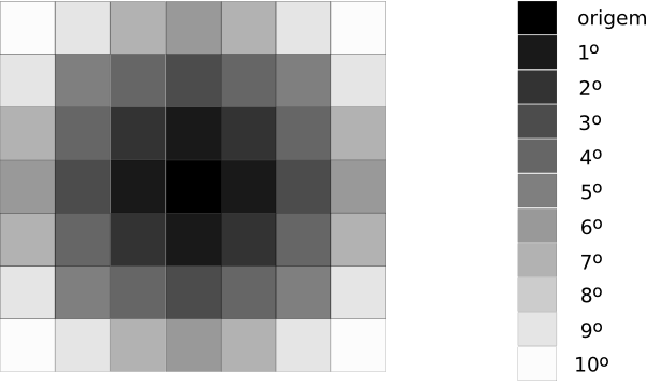
\includegraphics[width=0.33\textwidth]{vizinhos}
\end{center}
\renewcommand{\figurename}{Figura}
\caption{ {\small Ordenamento dos sítios vizinhos na rede.}}
\label{vizinho_fig}
\end{figure}

Tendo isso em vista, a partir, respectivamente, das somas direta e recíproca da equação (\ref{utotal3}), definimos as seguintes funções acumuladas $h_{n}$ e $g_{m}$:
\begin{equation}
h_{n}=\sum_{t=1}^{n} \frac{C_{t}}{r_{t}^{3}} \left[ \text{erfc} \left( \eta \frac{r_{t}}{L} \right) + \frac{2 \eta}{\sqrt{\pi}} \frac{r_{t}}{L} e^{-\eta^{2} \left( \frac{r_{t}}{L}\right)^{2}} \right]
\nonumber
\end{equation}
e
\begin{eqnarray*}
g_{m}= ~~~~~~~~~~~~~~~~~~~~~~~~~~~~~~~~~~~~~~~~~~~~~~~~~~~~
\\ \frac{2 \pi}{L^{3}} \sum_{t=0}^{m} C_{t} \left[ \frac{2 \eta}{\sqrt{\pi}} \,   e^{-\frac{\pi^{2} k_{t}^{2}}{\eta^{2}}} - 2 \pi k_{t} ~ \text{erfc} \left( \frac{\pi k_{t}}{\eta} \right) \right]
\\= \frac{2 \pi}{L^{3}} ~ \tilde{g}_{m} ~ ,
~~~~~~~~~~~~~~~~~~~~~~~~~~~~~~~~~~~~~~~~~~~~
\end{eqnarray*}
onde $r_{t}$ e $k_{t}$ são as distâncias discretas (em unidades de comprimento) do $t$-ésimo vizinho e $C_{t}$ é o número de vizinhos a uma distância $r_{t}$ (ou $k_{t}$). A Tabela 1 mostra os quatro primeiros valores de $C_{t}$, $r_{t}$ e $k_{t}$.
Os valores de $n$ e $m$ determinam o número de termos somados em cada série.

\begin{table}[h]
\begin{center}
\begin{tabular}{l c c} \hline
~~~ $t$ & $C_{t}$ & $r_{t}$, $k_{t}$\\
\hline
~~~ 1 & 4 & 1,0000\\
~~~ 2 & 4 & 1,4142\\
~~~ 3 & 4 & 2,0000\\
~~~ 4 & 8 & 2,2461\\
~~~ \vdots & \vdots & \vdots\\
\hline
\end{tabular}
\caption{ {\small Número de vizinhos $C_{t}$ à uma distância $r_{t}$, $k_{t}$.}}
\end{center}
\label{tabela_dos_vizinhos}
\end{table}
\vspace*{-0.6cm}

Vale notar que $h_{n}$ tem uma dependência em relação ao tamanho do sistema $L$, o que não existe para $\tilde{g}_{m}$.

Para determinarmos $r_{\min}$ e $k_{\min}$ definimos os erros relativos para $h_{n}$ e $\tilde{g}_{m}$, respectivamente, como:
\begin{eqnarray*}
\varepsilon_{n} = \frac{\left| h_{n \rightarrow \infty}-h_{n} \right|}{|h_{n \rightarrow \infty}|}
\end{eqnarray*}
e
\begin{eqnarray*}
\varepsilon_{m} = \frac{\left| \tilde{g}_{m \rightarrow \infty}-\tilde{g}_{m} \right|}{|\tilde{g}_{m \rightarrow \infty}|} ~~ \text{.}
\end{eqnarray*}

Os valores mostrados para $r_{\min}/L$ e $k_{\min}$ nas Figuras \ref{rmax_L} e \ref{kmax_eta} foram obtidos impondo que o erros relativos $\varepsilon_{n}$ e $\varepsilon_{m}$ sejam no máximo $10^{-5}$.

\begin{figure}[!ht]
\centering
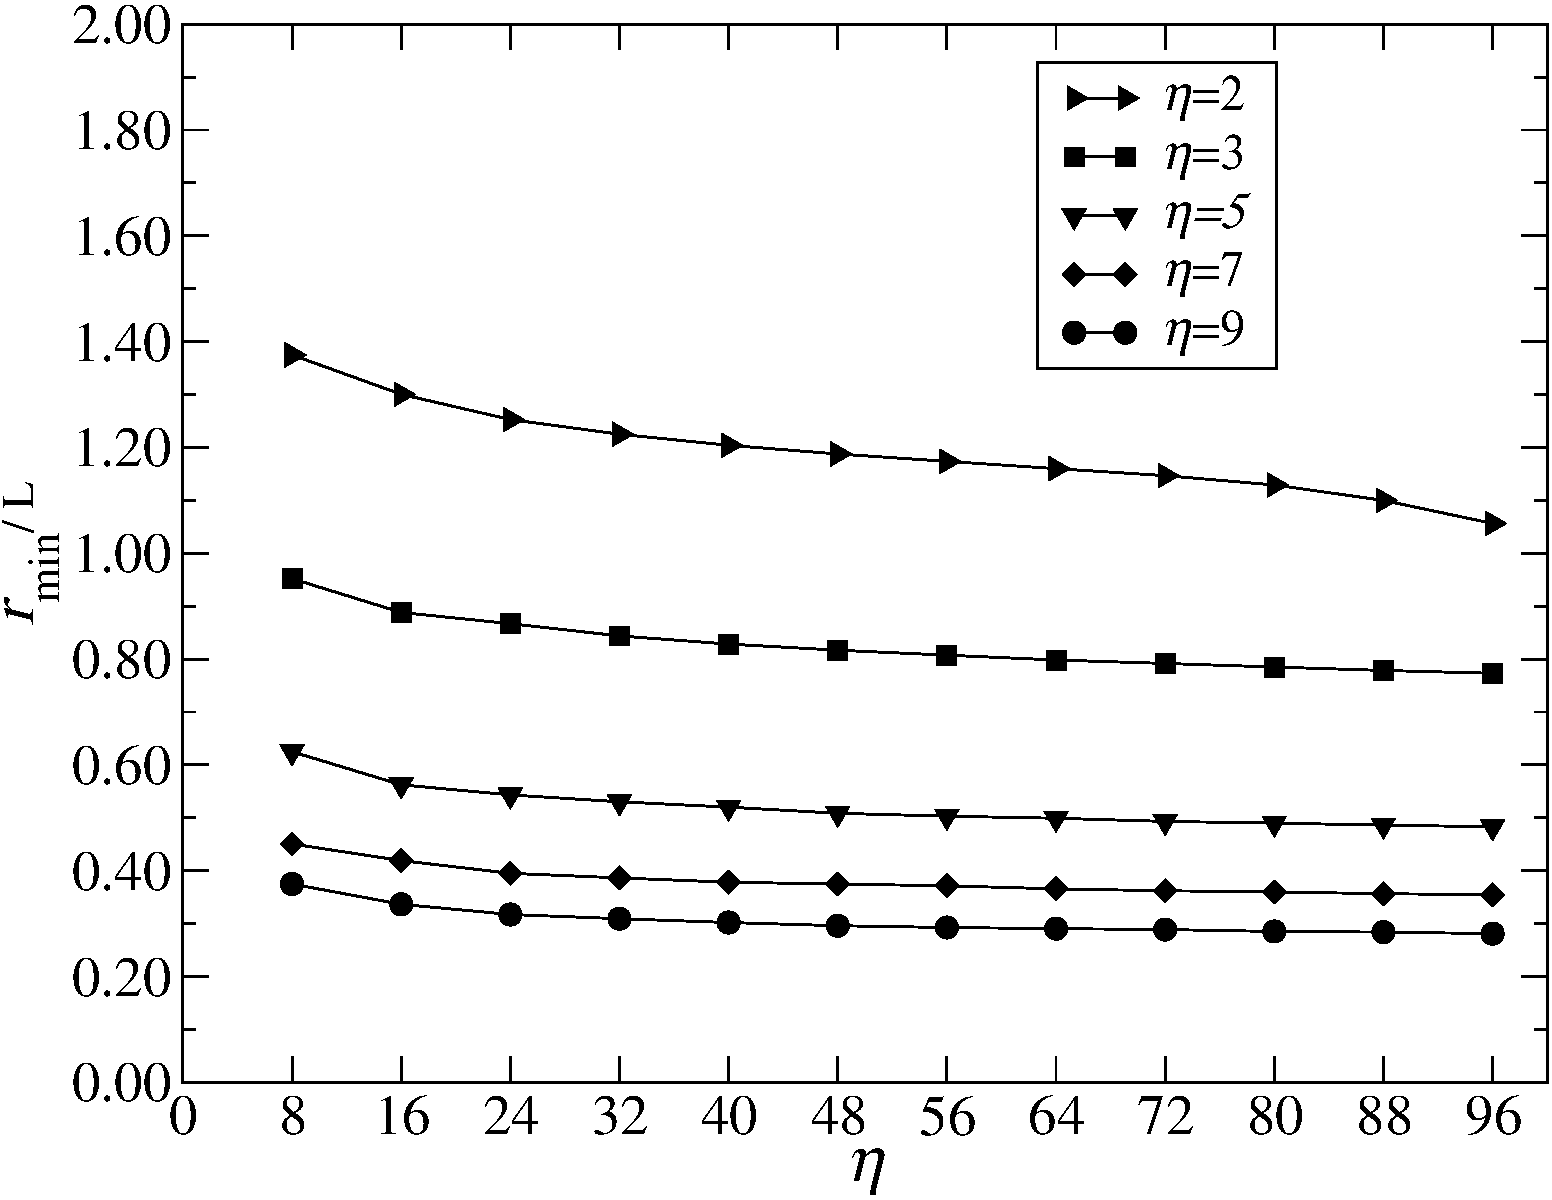
\includegraphics[width=0.45\textwidth]{rmin}
\renewcommand{\figurename}{Figura}
\caption{ {\small Gráfico de $r_{\min}/L $ por $L$ para diferentes valores de $\eta$.}}
\label{rmax_L}
\end{figure}

A Figura \ref{rmax_L} mostra que o aumento no parâmetro $\alpha$ (aumento em $\eta$) causa diminuição no parâmetro $r_{\min}/L$, auxiliando a convergência da série. Observamos também o efeito do tamanho do sistema sobre $r_{\min}/L$: à medida que $L$ aumenta, a razão $r_{\min}/L$ diminui.

\begin{figure}[!b]
\centering
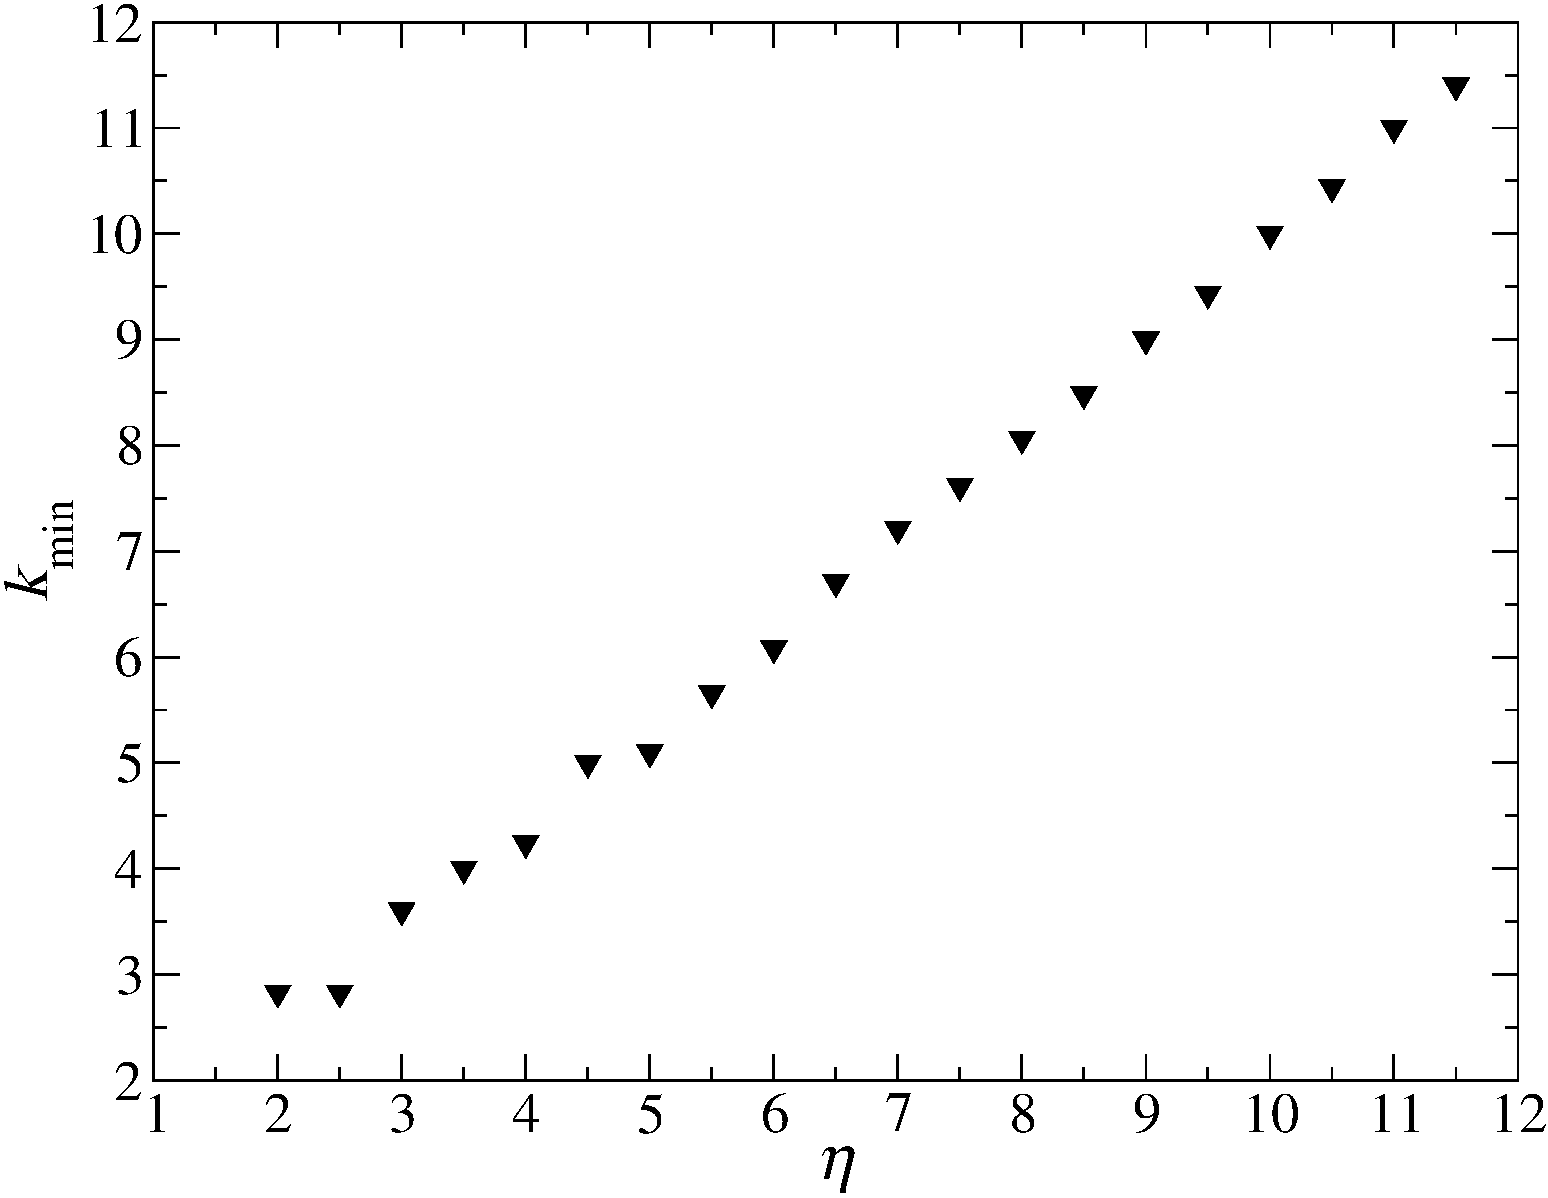
\includegraphics[width=0.45\textwidth]{kmin}
\renewcommand{\figurename}{Figura}
\caption{ {\small Gráfico de $k_{\min}$ por $\eta$.}}
\label{kmax_eta}
\end{figure}

Na Figura \ref{kmax_eta} observamos a dependência linear de $k_{\min}$ com $\eta$.

Como aplicação do efeito dos parâmetros analisados acima, calculamos a energia de interação dipolar. Para isso, consideramos um sistema com $N=1024$ partículas ($L=32$), $q_{i}=1$ ($i=1,...,N$), $g=\frac{1}{2}$ e utilizamos a expressão (\ref{utotal_c_s}) ($p=3$), atribuindo diversos valores à $\eta$. Os resultados são apresentados na Tabela 2. Esta tabela mostra a relação entre os parâmetros para obtermos uma precisão pré-estabelecida no cálculo da energia de interação por partícula.

\begin{table}[h]
\begin{center}
\begin{tabular}{c c c c} \hline
$\eta$ & $U_{\text{dipolar}}^{(3)}/N$ & $r_{\min}$ & $k_{\min}$\\
\hline
 3.0 & $4.51679\,91$ & 27 & 5  \\
 3.5 & $4.51680\,37$ & 24 & 5  \\
 4.0 & $4.51680\,31$ & 21 & 5  \\
 4.5 & $4.51680\,47$ & 19 & 6  \\
 5.0 & $4.51680\,38$ & 17 & 6  \\
 5.5 & $4.51680\,69$ & 16 & 7  \\
 6.0 & $4.51680\,81$ & 15 & 7  \\
 6.5 & $4.51680\,86$ & 14 & 8  \\
 7.0 & $4.51680\,86$ & 13 & 8  \\
 7.5 & $4.51680\,81$ & 12 & 9  \\
 8.0 & $4.51680\,66$ & 11 & 9  \\
 8.5 & $4.51680\,95$ & 11 & 9  \\
 9.0 & $4.51680\,81$ & 10 & 10 \\
 9.5 & $4.51680\,99$ & 10 & 10 \\
10.0 & $4.51680\,82$ & 9  & 11 \\
\hline
\end{tabular}
\caption{ {\small Valores da energia total de interação dipolar $U_{\text{dipolar}}^{(3)}/N$ ($L=32$) e os respectivos valores de $r_{\min}/L$ e $k_{\min}$ em função de $\eta$.}}
\end{center}
\label{tabela_dos_vizinhos}
\end{table}
\vspace*{-0.6cm}

\begin{thebibliography}{10}
\bibitem{EWA}
P. P. Ewald, Die Berechnung optischer und elektrostatischer Gitterpotentiale, {\em Annalen der Physik}, 369 (1921) 253-287.

\bibitem{GAO}
G. T. Gao e X. C. Zeng, Vapor-liquid coexistence of quasi-two-dimensional Stockmayer fluids {\em J. Chem. Phys.}, 106 (1997) 3311-3317.

\bibitem{GRAD}
I. S. Gradshteyn e I. M. Rhyzik, Tables of integrals, series and products, Academic, New York, 1980.

\bibitem{NIJ}
B. R. A. Nijboer e F. W. De Wette, On the calculation of lattice sums, {\em Physica}, 23 (1957) 309-321.

\end{thebibliography}

\end{document}
